% Informationen zu den Öffnungszeiten.
% http://www.math.uni-hamburg.de/home/jampert/formulare/index_o.html#oeffnung-cip
\subsection{CIP-Pool}

Am Fachbereich Mathematik stehen euch auch Arbeitsplätze zur Verfügung, die mit
einem Computer ausgestattet sind. Diese findet ihr in den sogenannten
CIP-Pools, die sich in der ersten Etage des Geomatikums befinden. Neben einer
großen Zahl von Computern mit Betriebssystem Windows gibt es auch einige
Computer auf denen UNIX als Betriebssystem installiert ist. Sämtliche Computer
sind mit mathematischer Software, einem Zugang zum Internet und einem
persönlichen Speicherplatz ausgestattet.

\subsubsection{Zugang zu den Computern}

Die Räume des CIP-Pools sind sowohl in der Vorlesungszeit als auch in den
Semesterferien regelhaft von 10:00 bis 16:00 Uhr geöffnet. Die Öffnungszeiten
werden nicht all zu streng gesehen, sodass es einerseits häufig kein Problem
ist, länger zu arbeiten, andererseits die Verfügbarkeit nicht unbedingt immer
um 10:00 Uhr beginnt. Im letzteren Fall lohnt es sich häufig im selben
Stockwerk beim Verwaltungspersonal nachzufragen, ob die Räume aufgeschlossen
werden können.

Um einen der Computer benutzen zu können, müsst ihr euch mit eurer persönlichen
Kennung anmelden. Diese wird euch auf dem Postweg mitgeteilt. Falls ihr eure
Zugangsdaten nicht erhalten haben solltet, so könnt ihr diese beim
Rechenzentrum, in der Schlüterstraße 70, oder bei den Aufsichten des CIP-Pools
beantragen. Die Bearbeitung nimmt allerdings mindestens einen Tag in Anspruch.
Eure Zugangsdaten bestehen aus einer persönlichen Kennung sowie einem Passwort.
Beim Anmelden an einem Computer müsst ihr zudem noch eine Nutzergruppe angeben,
die für Studenten des Fachs Mathematik oder Wirtschaftsmathematik \glqq
Studi\grqq, für Studenten des Lehramts mit Fach Mathematik \glqq Erzwiss\grqq\
lautet. Die Gruppe \glqq Mathe\grqq\ ist Mitarbeitern an der Fakultät
vorbehalten.

Nach einer ersten erfolgreichen Anmeldung empfiehlt es sich, das eigene
Passwort zu ändern. Das könnt ihr unter \url{http://www.rrz.uni-hamnburg.de}
$\rightarrow$ Benutzung des RRZ $\rightarrow$ Passwort tun. Achtet darauf, ein
ausreichend sicheres Passwort zu wählen!

%\begin{center}
%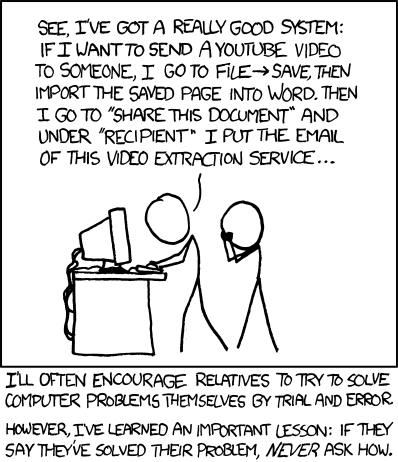
\includegraphics[scale=.2]{comics/763}
%\end{center}
%
%\begin{center}
%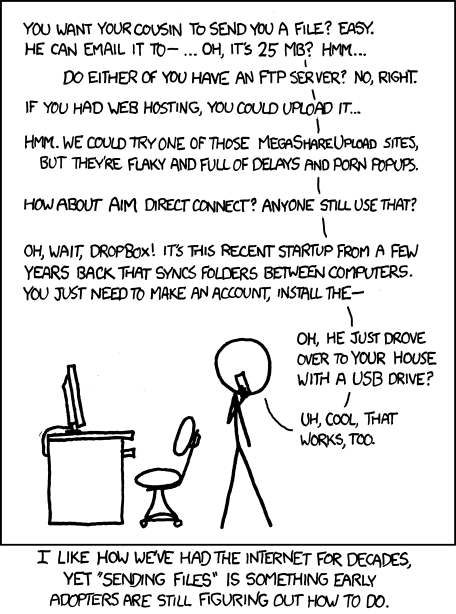
\includegraphics[scale=.2]{comics/949}
%\end{center}

\subsubsection{Speichern und Drucken}

Eines der leidigsten Themen an dem eigenen Laptop ist das Drucken in fremder
Umgebung. Dafür eignen sich die Computer in den CIP-Pools außerordentlich gut,
denn die Computer sind hier bereits konfiguriert und außerdem stellt der
Fachbereich Mathematik jedem Studenten ein monatliches Druckkontingent zur
Verfügung. Dieses kann an den Computern überprüft werden und durch einen
Druckauftrag an den Drucker l142, welcher sich -- wer hätte es geahnt -- im
Raum 142 befindet, in nahezu beliebig bedrucktes Papier verwandelt werden. Es
empfiehlt sich, im CIP-Pool nicht am letzt möglichen Tag und schon gar nicht im
letzt möglichen Moment etwas drucken zu wollen. Zu häufig hat man dafür mit den
üblichen Problemen -- kein Papier mehr, Düsen verstopft, Toner alle, keine
Netzwerkverbindung, Sanduhr, Sanduhr, Sanduhr, \dots -- zu kämpfen. In einem
solchen Fall wendet man sich am besten an die Aufsichten des CIP-Pools, die
sich entweder in den Computer-Räumen oder im Raum nebenan aufhalten.

Eines der leidigsten Themen an einem fremden Computer ist der Dateitransfer.
Glücklicherweise sind die Computer mit USB-Schnittstellen sowie einem
Netzlaufwerk ausgestattet, sodass man nicht voller Verlegenheit eine E-Mail an
sich selbst adressieren muss. Zudem besitzt jeder Student einen persönlichen
Speicherplatz von 20 MB, der von jedem Computer aus erreichbar ist und sobald
man sich anmeldet als ein Laufwerk (Windows) oder Mount-Point (UNIX)
eingebunden wird. Ihr solltet darauf achten, keine persönlichen oder wichtigen
Daten auf dem Computer außerhalb eures Netzlaufwerkes zu speichern. Zum einen
kann jemand, der den Computer nach euch benutzt, gegebenenfalls darauf
zugreifen. Zum anderen werden einige Speicherbereiche automatisch, andere
manuell durch die Administratoren gelöscht.

\subsubsection{E-Mail}

Jeder Student der Universität Hamburg erhält eine persönliche E-Mail-Adresse
nach dem folgenden Muster. Was passiert, falls zwei eingeschriebene Studenten
dieselben Namen aufweisen, haben wir leider noch nicht in Erfahrung bringen
können.

\url{vorname.nachname@studium.uni-hamburg.de}

Auf das Postfach dieser Adresse könnt ihr im Portal des Rechenzentrums
zugreifen. Dazu besucht ihr die Homepage des Rechenzentrums unter
\url{http://www.rrz.uni-hamburg.de} und wählt dort den Verweise auf Surfmail.
In dem folgenden Formular könnt ihr euch mit derselben Kennung anmelden, mit
der ihr die Computer in dem CIP-Pool nutzen könnt.
